\usetikzlibrary{arrows,positioning} 
\tikzset{
    %Define standard arrow tip
    >=stealth'
    }
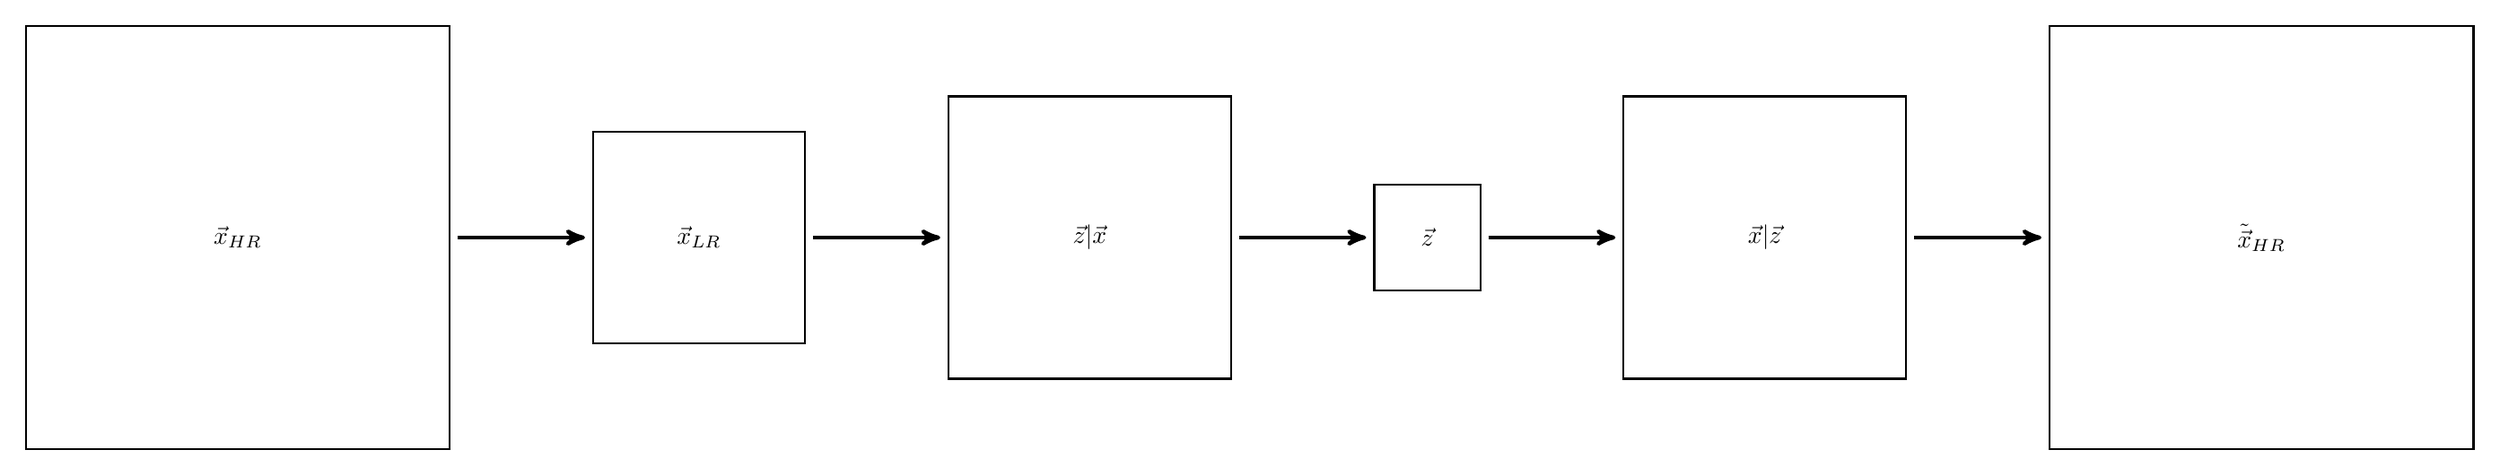
\begin{tikzpicture}[x = 1cm, y = 1cm, thick,
		image/.style={rectangle, draw, inner sep = 0pt, minimum size = 2 cm},
		network/.style={rectangle, draw, inner sep = 0pt, minimum size = 2 cm},
		arrow/.style={ ->, ultra thick, shorten <= 1 mm, shorten >= 1 mm}, node distance=2 cm
	]
	
	\node[image, minimum size = 6 cm] (HR) at (0, 0) {$\vec{x}_{HR}$};
	
	
	\node[image, minimum size = 3 cm, right = of HR] (LR) {$\vec{x}_{LR}$};
	
	
	\node[network, minimum size = 4 cm, right = of LR] (encoder) {$\enc{\vec{z}|\vec{x}}$};
		
	\node[network, minimum size = 1.5 cm, right = of encoder] (latent) {$\vec{z}$};
	
	
	\node[network, minimum size = 4 cm, right = of latent] (decoder) {$\dec{\vec{x}|\vec{z}}$};
		
	\node[image, minimum size = 6 cm, right = of decoder] (reconstruction) {$\tilde{\vec{x}}_{HR}$};
		
	\draw[arrow] (HR) -- (LR);
	\draw[arrow] (LR) -- (encoder);
	\draw[arrow] (encoder) -- (latent);
	\draw[arrow] (latent) -- (decoder);
	\draw[arrow] (decoder) -- (reconstruction);
	
\end{tikzpicture}
